
\section{Laser stand to test MAPMTs}
The large number if the channels in the RICG detector  poses challenging problem for the MAPMT testing and calibration.
RICH consists of 400 MAPMTs resulting in total number of channels equal to 25600. So in order to test them efficiently within a reasonable timeframe the fully automated test stand was build to evaluate 2 MAPMTs at once, with potential extension to 6 MAPMTs, as shown on Fig.~\ref{fig:MAPMTtest}.

\begin{figure}[hbt]
	\centering
	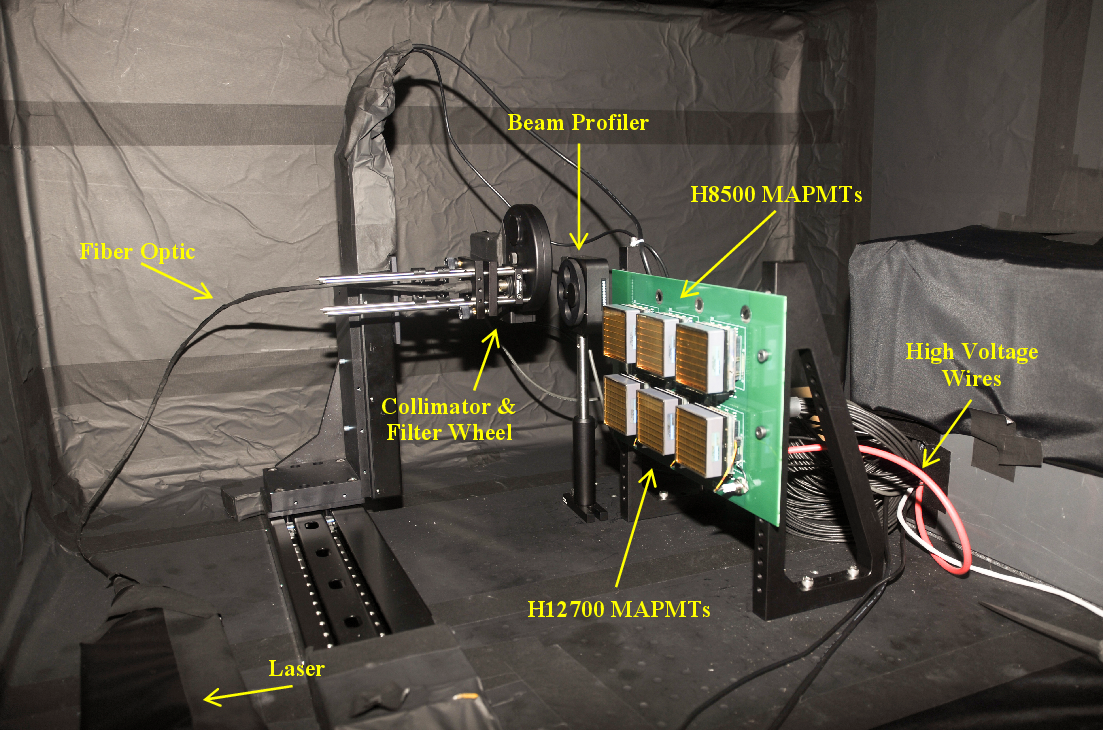
\includegraphics[width=0.9\linewidth]{blackbox.png}
	\caption{Evaluation setup.}
	\label{fig:MAPMTtest}
\end{figure}

The test stand consists of a 470 nm diode laser system, 2 long travel motorized stands to drive laser fiber in two dimensional space for individual pixel illumination, the motorized neutral density filter system, adapter board for MAPMT and JLab 250MHz FADC electronics for DAQ purposes.
The laser light is directed through the fiber and attenuated to the single photon level using the neutral density filters to mimic the conditions of the RICH detector.
The motors were remotely controlled to move the focused laser beam across (see Fig.~\ref{fig:beamopt1}) the entire surface of the MAPMT entrance window and illuminate one by one of all its 64 pixels individually.
Another option is to illuminate the whole surface of MAPMT photocathode at once using the Engineered Diffuser to produce square pattern with non-Gaussian intensity distribution (see Fig.~\ref{fig:beamopt2}).

\begin{figure}[bt]
	\centering
	\begin{subfigure}[b]{0.628\linewidth}
		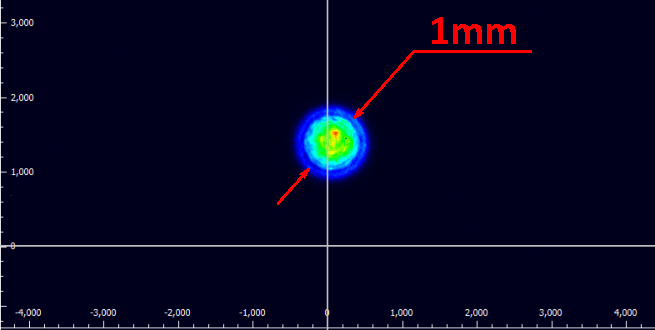
\includegraphics[width=\textwidth]{beamspot.pdf}
		\caption{Focused laser beam.}
		\label{fig:beamopt1}
	\end{subfigure}
	\begin{subfigure}[b]{0.354\linewidth}
		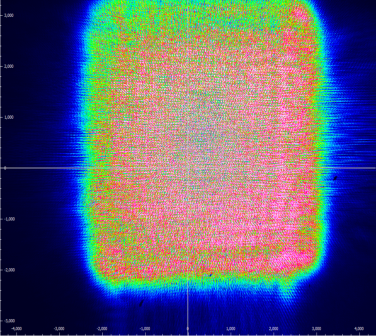
\includegraphics[width=\textwidth]{beamsquare.pdf}
		\caption{Square pattern.}
		\label{fig:beamopt2}
	\end{subfigure}
	\caption{The laser output options.}
\end{figure}

This configuration brings routine workload to minimum allowing the evaluation of 2 MAPMTs (equivalent to 128 conventional PMTs!) at 4 different high voltages and 6 different light intensities within 2 hours with less than 15 minutes of human intervention.

\begin{figure}[b]
	\centering
	\begin{subfigure}{0.3\linewidth}
		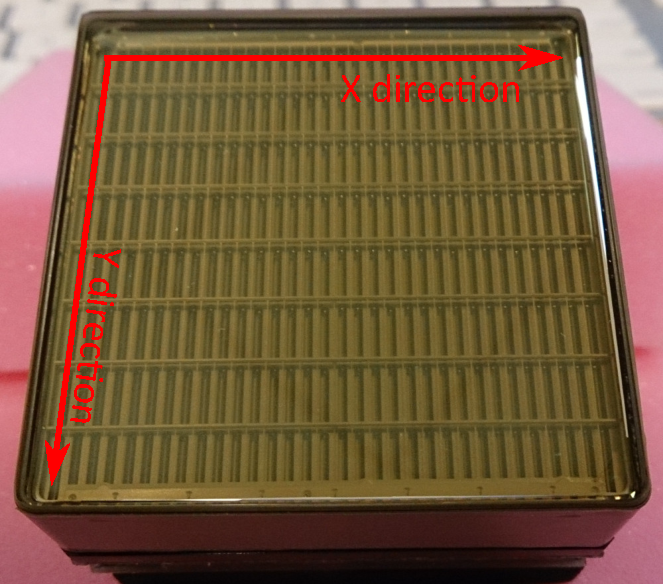
\includegraphics[width=\textwidth]{surfaceuniform1.pdf}
		\caption{MAPMT with visible internal structure of metal channel dynodes and focusing mesh.}
		\label{fig:surfaceuniform1}
	\end{subfigure}
	\quad
	\begin{subfigure}{0.3\linewidth}
		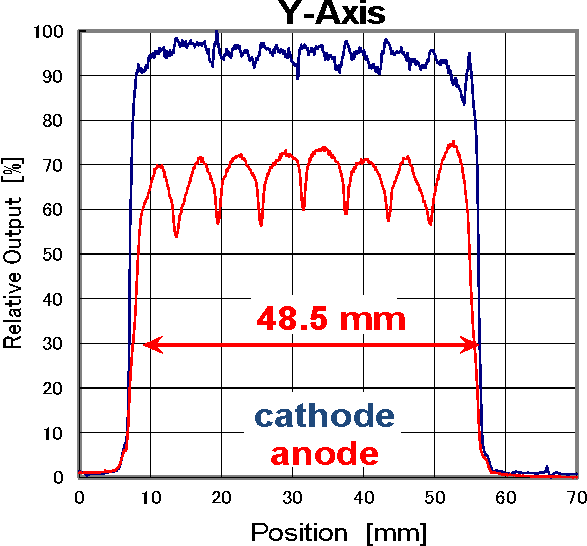
\includegraphics[width=\textwidth]{surfaceuniform3.pdf}
		\caption{The response along the X axis; the signal drops in the deadspace between the pixels.}
		\label{fig:surfaceuniform2}
	\end{subfigure}
	\quad
	\begin{subfigure}{0.3\linewidth}
		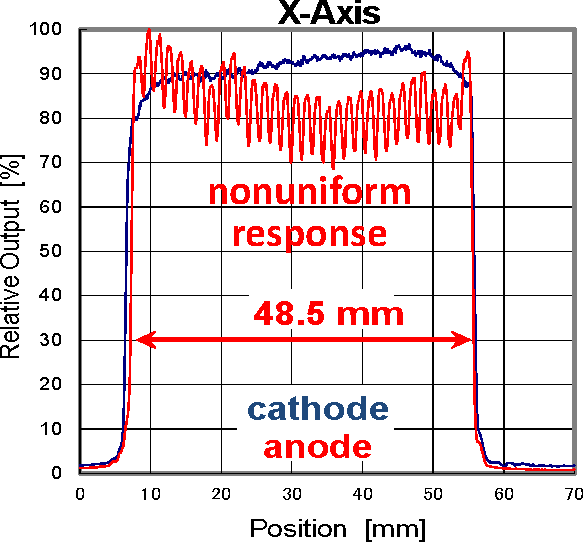
\includegraphics[width=\textwidth]{surfaceuniform2.pdf}
		\caption{The response along the Y axis: multiple segmentations within the pixels.}
		\label{fig:surfaceuniform3}
	\end{subfigure}
	\caption{The response uniformity of MAPMT.}
	\label{fig:surfaceuniform}
\end{figure}


Before starting the systematic study of the MAPMT responses, a finer two dimensional scan of several pixels was performed in order to verify the uniformity of the response across pixel's surfaces, as shown on Fig.~\ref{fig:surfaceuniform}.
The horizontal and vertical axes denote laser beam position during the scan.
Along the both directions there are obvious drops in efficiency when the laser strikes the space between the pixels.
The drops are relatively fast so the deadspace is very small as expected from the Hamamatsu specifications.
Additionally there exists a vertical efficiency variation across the pixel in horizontal scan.
These inhomogeneties are correlated with the vertical walls separating dynode chains, owing to the constructional features of the MAPMT. The discontinuity in dynode structure is visible from the MAPMT photon on Fig.~\ref{fig:surfaceuniform1}.
The separate response maps for photocathode shows relatively uniform signal without efficiency drops, confirming that the variation arises from the dynode system.
